\documentclass[a4paper]{article}

\usepackage[utf8]{inputenc}
\usepackage[T1]{fontenc,url}
\usepackage{cite}
\usepackage{hyperref}
\usepackage{amsmath, amssymb}
\usepackage{tikz}
\usepackage{graphicx}
\usepackage{parskip}
\usepackage{lmodern}
\usepackage{algorithm}
\usepackage{algpseudocode}
\usepackage{epigraph}


\begin{document}
\title{FYS3150 -- Project 1}
\author{
    \begin{tabular}{r l}
        Kristian Gregorius Hustad & (\texttt{krihus})\\
        Jonas Gahr Sturtzel Lunde & (\texttt{jonassl})
    \end{tabular}}
%\date{}    % if commented out, the date is set to the current date

\maketitle



% quote
\setlength{\epigraphwidth}{0.75\textwidth}
\renewcommand{\epigraphflush}{center}
\renewcommand{\beforeepigraphskip}{50pt}
\renewcommand{\afterepigraphskip}{100pt}
\renewcommand{\epigraphsize}{\normalsize}
%\epigraph{The first principle is that you must not fool yourself -- and you are the easiest person to fool.}{\textit{Richard Feynman}}

\epigraph{With Python, life is much simpler.}{\textit{Morten Hjorth-Jensen}}

\begin{abstract}
TODO
\end{abstract}

\vfill


\begin{center}
    GitHub repository at \url{https://github.com/KGHustad/FYS3150}
\end{center}

\newpage

%%% MACROS
\newcommand{\half}{\frac{1}{2}}
\newcommand{\dx}{{\Delta x}}



\section{Introduction}
%\subsection*{Description of the nature of the problem}

In this project, we aim to find a numerical solution to the following ODE with Dirichlet boundary conditions
\begin{equation}
    -u''(x) = f(x), \quad x\in(0,1), \quad u(0) = u(1) = 0
    \label{eq:ddu_dxx_cont}
\end{equation}

where the source term, $f(x)$, is a known function.

We derive a numerical scheme, which we solve as a matrix equation, by viewing the scheme as a set of linear equation, which can be mapped onto a tridiagonal matrix. We devise a general solution by gaussian elimination, which we then specialize, and lastly we solve the matrix equation by LU-factorization.

In section \ref{sec:methods}, we derive and analyze the algorithms, and in section \ref{sec:implementation_and_results}, we discuss the implementation and analyze the performance of the algoritms. Finally, a conclusion is given in section \ref{sec:conclusion}.

\section{Discussion of methods}\label{sec:methods}
\subsection{An analytical solution}

With the source term
\begin{equation}
    f(x) = 100e^{-10x}
    \label{eq:f_analytical}
\end{equation}

there exists an analytical solution
\begin{equation}
    u(x) = 1-(1-e^{-10})x-e^{-10x}
    \label{eq:u_analytical}
\end{equation}

We should verify that \eqref{eq:u_analytical} with the source term \eqref{eq:f_analytical} is in fact a solution to \eqref{eq:ddu_dxx_cont}.

\begin{align*}
    \frac{d^2}{dx^2}  u(x)
    &= \frac{d^2}{dx^2} \left( 1-(1-e^{-10})x-e^{-10x} \right) \\
    &= \frac{d}{dx} \left( (1-e^{-10})+10e^{-10x} \right) \\
    &= -100e^{-10x} \\
    &= -f(x) \\
    u(0)
    &= 1-(1-e^{-10})\cdot 0-e^{-10 \cdot 0} \\
    &= 1-0-1 \\
    &= 0 \\
    u(1)
    &= 1 - (1-e^{-10}) - e^{-10} \\
    &= 1 - 1 + e^{-10} - e^{-10} \\
    &= 0
\end{align*}

We see that \eqref{eq:u_analytical} and \eqref{eq:f_analytical} satifies \eqref{eq:ddu_dxx_cont}, hence we do indeed have an analytical solution.
This analytical solution will be used in the rest of this project to assert the correctness and measure the rate of convergence of our numerical approximations.
Therefore, it is instructive to plot the exact solution here, before we proceed into the inexact realm of numerics.

% \begin{figure}[ht]
% \begin{center}
% \begin{tikzpicture}[scale=6]
%     \draw[step=0.1, gray, very thin] (0,0) grid (1, 1);
%     \draw [domain=0:1] plot (\x, {1 - (1-exp(-10)) * \x - exp(-10 * \x)});
% \end{tikzpicture}
% \end{center}
% \caption{Plotting \eqref{eq:u_analytical} with Wolfram Alpha}
% \end{figure}

%\begin{figure}[ht]
%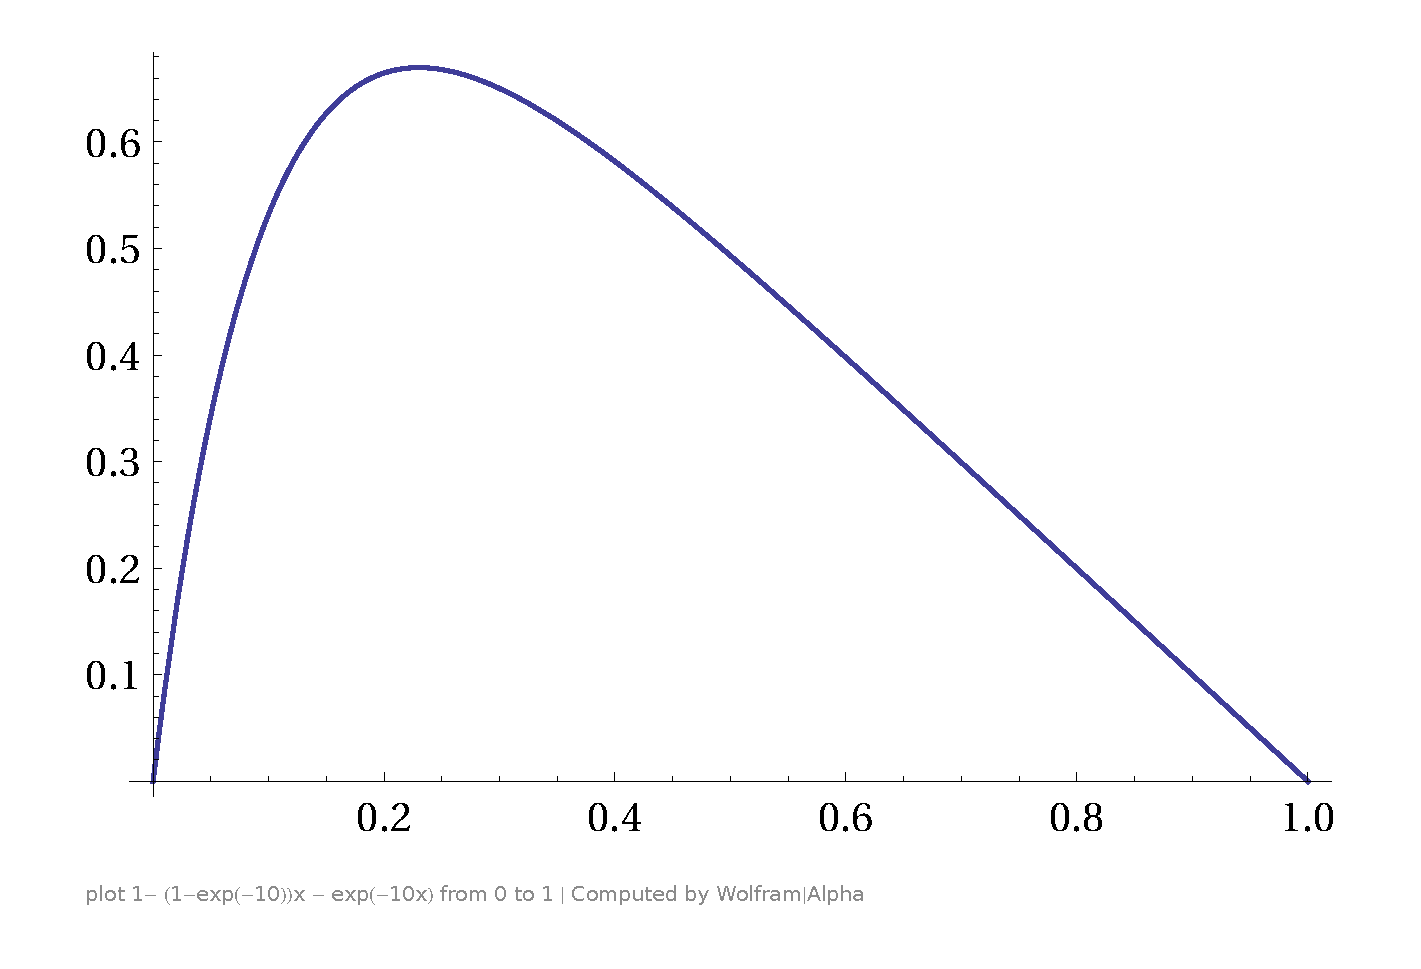
\includegraphics[width=\textwidth]{fig/exact_solution_wolfram_alpha_plot}
%\caption{Plotting \eqref{eq:u_analytical} with Wolfram Alpha}
%\end{figure}

\begin{figure}[ht]
\includegraphics[width=\textwidth]{fig/plot_exact}
\caption{Plotting the analytical solution, \eqref{eq:u_analytical}}
\end{figure}

\subsection{Deriving a numerical scheme}
Deriving a numerical scheme for solving \eqref{eq:ddu_dxx_cont} by the finite difference method is rather trivial.
We discretize $u(x), \quad x \in [0, 1]$ as $n+2$ ($n$ excluding the boundaries) equally spaced points $v_0, \dots, v_{n+1}$. To denote the set of indices for the points, we employ notation from \cite{hpl_fdm} and introduce $\mathcal{I} = \{ i \mid i \in \mathbb{Z}, 0 \leq i \leq n + 1\}$ and for the inner points (viz. excluding the boundaries) $\mathcal{I}_i = \{ i \mid i \in \mathbb{Z}, 0 < i < n + 1\}$.
The boundary conditions imply
\begin{equation}
v_0 = v_{n+1} = 0
\label{eq:boundaries_disc}
\end{equation}
The source term, $f(x), \quad x \in [0, 1]$ is discretized similarly. We can discretize \eqref{eq:ddu_dxx_cont} as

\begin{align*}
-[D_x D_x u]_i &= f_i \\
\frac{-1}{\dx} \left( [D_x u]_{i+\half} - [D_x u]_{i-\half} \right) &= f_i \\
\frac{-1}{\dx} \left( \frac{v_{i+1} - v_{i}}{\dx} - \frac{v_{i} - v_{i-1}}{\dx} \right) &= f_i \\
\frac{-1}{\dx^2} \left( v_{i+1} - 2v_{i} + v_{i-1} \right) &= f_i \\
-v_{i+1} + 2v_{i} - v_{i-1}  &= \dx^2 f_i
\end{align*}

where $i \in \mathcal{I}_i$. Setting $h = \dx$, we obtain the following equation

\begin{equation}
-v_{i+1} + 2v_{i} - v_{i-1}  = h^2 f_i, \quad i \in \mathcal{I}_i
\label{ddu_dxx_disc}
\end{equation}

This corresponds to a system of linear equations where the unknowns are $v_i, \quad i \in \mathcal{I}_i$. To save space, we introduce $s_i = h^2 f_i, i \in \mathcal{I}_i$.

\begin{equation}\label{eq:sys_lin_eq}
    \begin{array}{cccc}
        a_1 v_{0} + b_1 v{1} + c_1 v_{2} &= s_1 \\
        a_2 v_{1} + b_2 v{2} + c_2 v_{3} &= s_2 \\
        \vdots \\
        a_n v_{n-1} + b_n v{n} + c_n v_{n+1} &= s_n \\
    \end{array}
\end{equation}

In our scheme,
\begin{equation}
a_i = -1, b_i = 2, c_i = -1 \quad \forall \quad i \in \mathcal{I}_i
\label{eq:spec_abc}
\end{equation}
but we will extend the theory to a more general case.

Being a system of linear equations, \eqref{eq:sys_lin_eq} can be rewritten as a matrix equation $A {\bf v} = {\bf s}$, where ${\bf v} = (v_1, \dots, v_{n})$, ${\bf s} = h^2 {\bf f} = (h^2 s_1, \dots, h^2 s_{n})$ and $A$ is a $n \times n$ matrix defined as

\begin{equation}
     A = \left(\begin{array}{ccccccccc}
                   b_1 & c_1 & 0 &\dots   & \dots &\dots & \dots &\dots&\dots\\
                   a_2 & b_2 & c_2 & 0 &\dots &\dots & \dots&\dots&\dots \\
                   0 & a_3 & b_3 & c_3 & 0 & \dots & \dots&\dots&\dots \\
                   \vdots&\vdots&\vdots&\vdots&\vdots&\vdots&\vdots&\vdots&\vdots \\
                   \dots&\dots&\dots&\dots&\dots & 0 & a_{n-1}  &b_{n-1}& c_{n-1} \\
                   \dots&\dots&\dots&\dots&\dots&\dots &  0 &a_n & b_n \\
              \end{array} \right)
\end{equation}

Notice that $a_1$ and $c_{n}$ do not appear in the matrix although they are present in the system of equations. As a consequence of the boundary conditions, we have \eqref{eq:boundaries_disc}, which in turn implies $a_1 v_{0} = a_1 \cdot 0 = 0$ and $c_n v_{n+1} = c_n \cdot 0 = 0$, hence we can omit $a_1$ and $c_{n}$ from the matrix.



\subsection{A general algorithm for solving an equation with a tridiagonal matrix}\label{subsec:gen_alg}
We can solve $A {\bf v} = {\bf s}$ for any tridiagonal matrix $A$ with standard Gaussian elimination. Since most of the matrix elements are zero, we choose to represent the matrix as three arrays, \texttt{a}, \texttt{b}, and \texttt{c}. Additionally, $v_{i}$ and $s_i$ are stored in the arrays \texttt{v} and \texttt{s}, respectively.

\begin{algorithm}
\caption{Gaussian elimination for a tridiagonal matrix} \label{alg:gaussian-general-tridiagonal}
\begin{algorithmic}[1]
  \For {$i \gets 2, \dots, n$} \Comment{Forward substitution eliminating $a_i$}
    \State $b_i \gets b_i - c_{i-1}\cdot \frac{a_i}{b_{i-1}}$ \Comment{Update $b_i$}
    \State $s_i \gets s_i - s_{i-1}\cdot \frac{a_i}{b_{i-1}}$ \Comment{Update $s_i$}
    \State $a_i \gets a_i - b_{i-1}\cdot \frac{a_i}{b_{i-1}} = 0$ \Comment{Set $a_i$ to 0 (can be skipped)} \label{alg_line:update_a}
  \EndFor

  \Statex \Comment{Backward substitution obtaining $v_i$}
  \State $v_n \gets \frac{s_n}{a_n}$
  \For {$i \gets n-1, \dots, 1$}
    \State $v_i \gets \frac{s_i - b_i v_{i+1}}{a_i}$
  \EndFor
\end{algorithmic}
\end{algorithm}

We see that algorithm \ref{alg:gaussian-general-tridiagonal} requires a number of floating point operation on the order of $8n$ \footnote{To be precise, there are $(n-1)5 + 1 + (n-1)3 = 8n-7$ flops, but there is no point in fine counting the exact number, as the runtime will be dominated by the leading term, $8n$.}, provided that we avoid computing the ratio $\frac{a_i}{b_{i-1}}$ twice and skip line \ref{alg_line:update_a}.
We also note that the space requirements are on the order of $5n$.

\subsection{A more specialized algorithm}
In \ref{subsec:gen_alg}, we devised a \emph{general} algorithm, meaning we did not exploit the fact that $a_i=k_a, b_i=k_b, c_i=k_c \quad \forall \quad i \in \mathcal{I}_i$ where the constants $k_a$, $k_b$ and $k_c$ have values as in  \eqref{eq:spec_abc}.


\subsection{LU decomposition}


\section{Implementation and results}\label{sec:implementation_and_results}
We chose Python as our implementation language because it allows for rapid development and has a syntax which is very close to the algorithmic language we are translating from. For future project, we will consider using C++, but it's main advantage lies is the efficiency, which wasn't a big problem for our programs.

\begin{figure}[ht]
\includegraphics[width=\textwidth]{fig/plot_b}
\caption{Approximation to $u$ by algorithm \ref{alg:gaussian-general-tridiagonal}}
\end{figure}

\subsection{Studying the error}

\subsection{Efficiency}


\section{Conclusion}\label{sec:conclusion}

%\bibliographystyle{plain}
%\bibliographystyle{siam}
\bibliographystyle{IEEEtran}
\bibliography{papers}{}

\end{document}
